


%SK:  copied this text from source sited below. Can we plug it in to the very beginning of the proposal as an italicized/centered quote?
\begin{myquoting}{\cite{jaiswal2018participation}}

Deafblindness, also known as dual sensory loss, is a varying combination of visual and
hearing impairment in the same individual. Interest in this topic has increased recently due
to evidence suggesting an increase in prevalence of this condition among older adults. Persons with deafblindness frequently experience participation barriers and social isolation. Developing an understanding of their experiences can inform the design of programs and
policies to enhance participation of people with deafblindness in society .
\end{myquoting}

Individuals who are Deaf-blind represent a small percentage of the US population, but one with highly specialized transportation and navigational needs that are, to date, unmet. No current technology or apps communicate information about the layout of an environment in a manner that is easily and portably consumable by this cohort. Our proposal seeks to close this information gap and enable this community to create its own maps, rather than rely on a mediator, to decide what information is relevant to them. By doing so, we hope to lower or remove transportation barriers that prevent Deaf-blind persons from participating fully in society. 

\subsection{Problem: A Fundamental Communication Barrier With Significant Quality of Life Implications}

Maps are an important tool for navigation because they help people to understand the spatial layout of an environment. However, they are inherently visual and content-rich. One solution that has a long history in the Blind and Deaf-blind community is tactile maps – maps that use raised features to represent spatial layouts and landmarks. Common approaches include embossing, printing in Braille, and “swell” (microcapsule) paper. These approaches can be used to create a two-layer tactile visualization from an image (\textit{e.g.}, \cite{miele2006talking}).

However, maps created by these approaches suffer from some serious limitations. First, they can be very costly \cite{rice2005design}, are non-scalable, and the technology for creating them is not readily available. Second, they lack standardization as they are largely a reflection of work put forth by Orientation and Mobility specialists who do not envisage the work as traditional cartographers would \cite{lobben2012tactile, gual2012visual}. Third, they represent limited types of information because they lack the expressive range of a solution that can vary more in height; for example, one cannot represent elevation changes and finer grained qualities of pavements without explicitly writing them into the map. Further, feature density and selecting the map scale creates a significant problem in the physical manifestation of a map due to the minimum size required for a finger to sense a tactile feature. Finally, in the past, reliable stewards who were skilled in creating tactile maps chose the features they deemed important on the users’ behalf; this resulted in limited customizability and a complete lack of user agency in determining the type and the amount of information available on the map. 


More recently, digital cartographic solutions are replacing all other maps. These solutions have the important advantage of being maintainable with relevant up to date information about changing street environments and transit services. However, personalized navigational mobile apps, such as Directions on Google Maps \cite{GoogleMaps}, are fundamentally visual and generally exclude blind, low vision and Deaf-blind populations. Common solutions are Blind-Aware phone applications targeting Blind navigators, which are GPS programs that provide auditory turn-by-turn directions (but little information that allows for exploration). To use these apps, Deaf-blind people must translate auditory prompts to tactile messages via Braille displays; this way of consuming the auditory information from these apps has a significant usability drawback: Braille displays refresh slower than spoken content, and therefore the apps' auditory cues, which are often verbose and generated at a fast pace, are difficult to comprehend for users with a Braille display interface.  

\subsubsection{Design Criteria}
\label{sec:design-criteria}
In light of the preceding constraints and limitations of both digital and tactile paper approaches, to solve this critical communication problem, our solution has to meet the following six \textbf{design criteria}: 
\begin{itemize}
 \item The solution must be scalable, reproducible, and cost effective. 
 \item The solution must use the best available pedestrian-centered information and standard tactile symbols. 
 \item The solution must improve expressivity of tactile maps, enabling more information to be included in the same spatially compact touch real estate.
 \item The solution must be customizable to user-specified parameters (including purpose of travel, area of interest, and other user-specific travel preferences). 
 \item The solution must be provided in a simple, open interface, allowing users of all abilities to create and customize their own maps. 
 \item The solution must contain current mapping data, and be updatable or provide a way for Deaf-blind users to be made aware of changes to the landscape in the mapped region.
\end{itemize}
Significantly, our solution must address usability criteria pertaining to the user experience of interacting with both our interfaces and maps. 

\subsubsection{Development Objectives}
\label{sec:design-objectives}

Based on these criteria, our solution will focus on creating a human-centered smart toolset and a cost-effective service system that allows Deaf-blind users to produce customized, 3D printed tangible maps on their own. %We will use 3D printing to reduce costs and extend reach and scalability of tactile maps. 
Specifically, in our development project, we will address each criterion with the following \textbf{development activities}:

\begin{itemize}
    \item We will extend our aggregated accessibility map codebase to support a production-level pipeline that produces 3D printed map models thereby extending reach and scalability (while reducing costs) of tactile maps.  (Section \ref{sec:fabrication})
    \item We will use the OpenSidewalks pedestrian-centric data standard \cite{bolten2017} and standard tactile symbols (\cite{BANA}) to represent features in a replicable, pedestrian-appropriate manner.  (Section \ref{sec:mapping-data})
    \item We will use multi-variable optimization algorithms to balance information richness with tactile usability (to enable appropriate use and density of tactile real estate). (Section \ref{sec:optimize})
    \item We will use a parameterized cost function to accommodate the user’s custom requirements about the area of travel, type of travel, and user needs and preferences.  (Section \ref{sec:optimize})
    \item We will focus on building accessible, user-tested, and user-friendly interfaces that are integrated into our production-level accessible map, designing all exchanges to be easily navigable using a 14 cell portable Braille reader (the most constrained interface we know to be in use). (Section \ref{sec:accessmap-integration})
    \item We will create optional services that will let users: (1) have their model printed and sent to them (at cost), and (2) subscribe to email alerts regarding any changes to the mapped region in the digital map repositories. (Section \ref{sec:alerts})
\end{itemize}

Our solution combines simple, accessible interfaces with complex data integration and smart routing. To our users, the entire solution will be seamlessly presented in a workflow through which Deaf-blind pedestrians access a website, select the area of travel, the type of travel they wish to undertake in the area, and travel preferences. They are given the opportunity to verify the map location and features via non-visual, text-based exchange before downloading it for a specified duration or choosing to print the map. The entire exchange is enabled and specifically designed for a portable 14-cell Braille display. At the conclusion of the interaction, users can decide whether to subscribe to email alerts to keep their tactile maps current and serviceable. 

%SK paragraph
In sum, we intend to produce three main \textbf{project deliverables}: an accessible web interface that lets users customize and create their own maps; an algorithm for creating custom tactile maps that is seamlessly integrated into a current accessible map solution; and an email notification system informing users about changes to landscape and service modifications in a specified travel area. Using our tools, Deaf-blind pedestrians will finally be able to access current, relevant, pedestrian-centric digital map and transit information. By doing so, they will become stronger decision makers, more self-reliant travelers, and less socially isolated members of society.

\begin{comment}
In sum, we have three main \textbf{project deliverables}:
\begin{itemize}
    \item An \textit{accessible web interface }that lets users customize and create their own maps
\item An \textit{algorithm for creating custom tactile maps} that is seamlessly integrated into a current accessible map solution.
\item An \textit{email notification system} informing users about changes to landscape and service modifications in a specified travel area.
\end{itemize}
Using our tools, Deaf-blind pedestrians will finally be able to access current, relevant, pedestrian-centric digital map and transit information. By doing so, they will become stronger decision makers, more self-reliant travelers, and less socially isolated members of society. 
\end{comment}

\subsection{Population: Who is being impacted}
%Digital mapping technology has made a transformative difference in the manner people, particularly urban residents, tackle their daily navigational needs; many people use smart phones and mapping applications to plan trips using the most up-to-date information to ensure they get to their destinations quickly and safely. 
More than 160 million blind, low-vision, and deaf-blind people worldwide have not realized the full potential of digital maps. 
%People in these groups often use special-purpose portable devices to solve specific map accessibility problems, such as finding location information via an external GPS device, and accessing printed text using optical character recognition (OCR).
Our primary focus will be on Deaf-blind individuals. Although few estimates of the global deaf-blind population exist, the population in the United States alone is believed to be at least 50,000 
(comprising of about 10,000 children and 43,000 adults) \cite{NCDB} and likely much larger because many in this
population identify with only their dominant impairment. For example, the Board of Directors of the National Association of Regulatory Utility Commissioners, convened in 2008, estimated between 70-100,000 of their consumers are Deaf-blind \cite{NARUC}.
%About 35-40,000 Americans are Deaf-blind \cite{watson1993model}, and 
Prevalence is higher among the elderly population, and with this demographic increasing, so has the population of Deaf-blind in the U.S. been increasing. This group's needs are often not considered in the design of technology, which may be accessible to blind, or Deaf persons, but not both. 

Although our focus is on Deaf-blind, it is worth noting that tactile maps are also of great interest for the Blind, and indeed the National Federation for the Blind has published a report on tactile graphics \cite{lobben2015tactile}. 3\% of Americans are legally blind (3.4 million people); vision loss is among the top 10 disabilities.
Thus our work will have impact both on an important and understudied smaller group (Deaf-blind) and also serve the needs of a much larger group. 


\subsection{Importance: Significant Unmet Barrier}

% Trying to drive home that there's no other option (tactile iPads aren't here yet and additive manufacturing is growing everywhere.
% Also drive home how dire the current situation is
For people who are Deaf-blind, unmet transportation needs pose a major barrier to accessing every facet of social participation, including access to on-location employment, healthcare resources, education, financial resources and community participation. 
Among these, participation in the workforce is one of the most important because of its ongoing impact on financial independence and social inclusion, and it is particularly limited for Deaf individuals and Blind individuals \cite{zwerling2002workforce}.  
In 2012, half of the individuals with a disability who were not working reported ``Lack of transportation'' as the third greatest barrier to work, following only ``one's own disability'' and ``lacking training'' \cite{BLS}.
Workforce inclusion aside, a lack of mobility has been generally linked to social exclusion \cite{kenyon2002transport}.


% AC: do we need to explain why social exclusion is a problem?

Trip planning (whether for navigating to a specific destination, for taking a multi-modal trip or for exploration) is a critical link in the complete door-to-door trip \cite{AttriCompleteTrip}, and is especially important to people who are Deaf-Blind, for whom minute changes even on a well-practiced route may completely subvert a trip.  Lack of reliable, current, sufficiently detailed information about transportation networks and pedestrian routing constitute a major part of the mobility problem for all people with special travel needs. However, efforts to ameliorate this problem today are largely focused around improving and building out the digital cartography infrastructure where the visual or audio experience of maps ranks above all senses. The concerns is that all the emerging data-driven, dynamic and engaging forms of mapping being produced today provide exclusively audio-visual articulations of the environment, thereby excluding Deaf-blind individuals and further hindering the downstream development of services and applications that could address the transportation needs of this cohort. 

There is data-supported recognition that this problem requires attention.
The Accessible Transportation Technology Research Initiative (ATTRI) studied the transportation challenges of people with all types of disabilities and identified significant unmet barriers to using transit, user needs when taking transit, and the most common issues with technology.
Of the three running examples of needed assistive technology solutions to address barriers associated with access to information, two were 
``tactile navigation/information device for individuals who are deaf-blind'' and ``proximity-based public announcements through text-based messaging'' alerting people about current conditions on the ground. Our work proposes a solution to address both.

In sum,  aids that meet the trip planning and navigational needs of Deaf-blind individuals are limited, and by our estimation, few are under development.
Thus, we must consider how experiences for people with both vision and hearing loss can be sensitively designed to provide comfortable, safe and delightful experiences mediating both destination-directed travel and exploration of the urban environment. 



\subsection{Broader Impact}
We believe this development project could benefit downstream creation of other products for individuals with disabilities.
The Tactile Map Tile application will be built using relatively inexpensive and scalable technology and open data sets (e.g., transit data APIs, OpenSidewalks data, and OpenStreetMap infrastructure), and could therefore be used and consumed in other applications. 
This data and tools can benefit municipalities and transit agencies by helping shift passengers with disabilities onto fixed‐route transit. 
Because ADA paratransit is 7‐to‐10 times more expensive per passenger trip than fixed route transit \begin{comment}

{(citation)}\end{comment}, any shift in passenger travel from paratransit to fixed‐route transit helps transit agencies control and potentially reduce operating and capital costs associated with
operating paratransit service. 
Upon completion, our application source code will be available using existing standards in open‐source development.
Tactile Map Tile will provide an affordable, reproducible, informative map artifact and the outcomes of this project will result in beneficial lessons, methodologies and tools that can be applied by transportation service providers in many regions, helping to attract and retain new travelers with and without disabilities.


\subsection{Preliminary Development: Proof of Concept Elucidated Needs of Mitigating Daily Exclusion}
\label{sec:pilot}

\begin{comment}

{the outcomes of this section are:
(1) explain that we have deep reach into this community already. 27 DB in this area out of the known 40 adults in Seattle, is pretty huge.
(2) that we were able to assess needs with the population and one of the outcomes was identifying the information types that we need to map for them, including everything that is found in the mapping-data section.
(3) that we found participants needed solutions to enable greater independence in navigation, wayfinding and exploration.
(4) that participants needed to be kept up to date on changes in their environment because they won't just be able to see it.
(5) that success will really depend on how well we integrate what we provide with the devices they already have, and the most limiting one is a 14 cell Braille reader so we should design for that. The Ladner study also supports this.
}
\end{comment}

Pairing a participatory, data-driven design approach together with interdisciplinary collaboration, we previously created 3D printed, parametrically designed maps to elicit feedback from Orientation and Mobility Specialists and would-be users who are Deaf-blind.


\begin{figure}
    \centering
    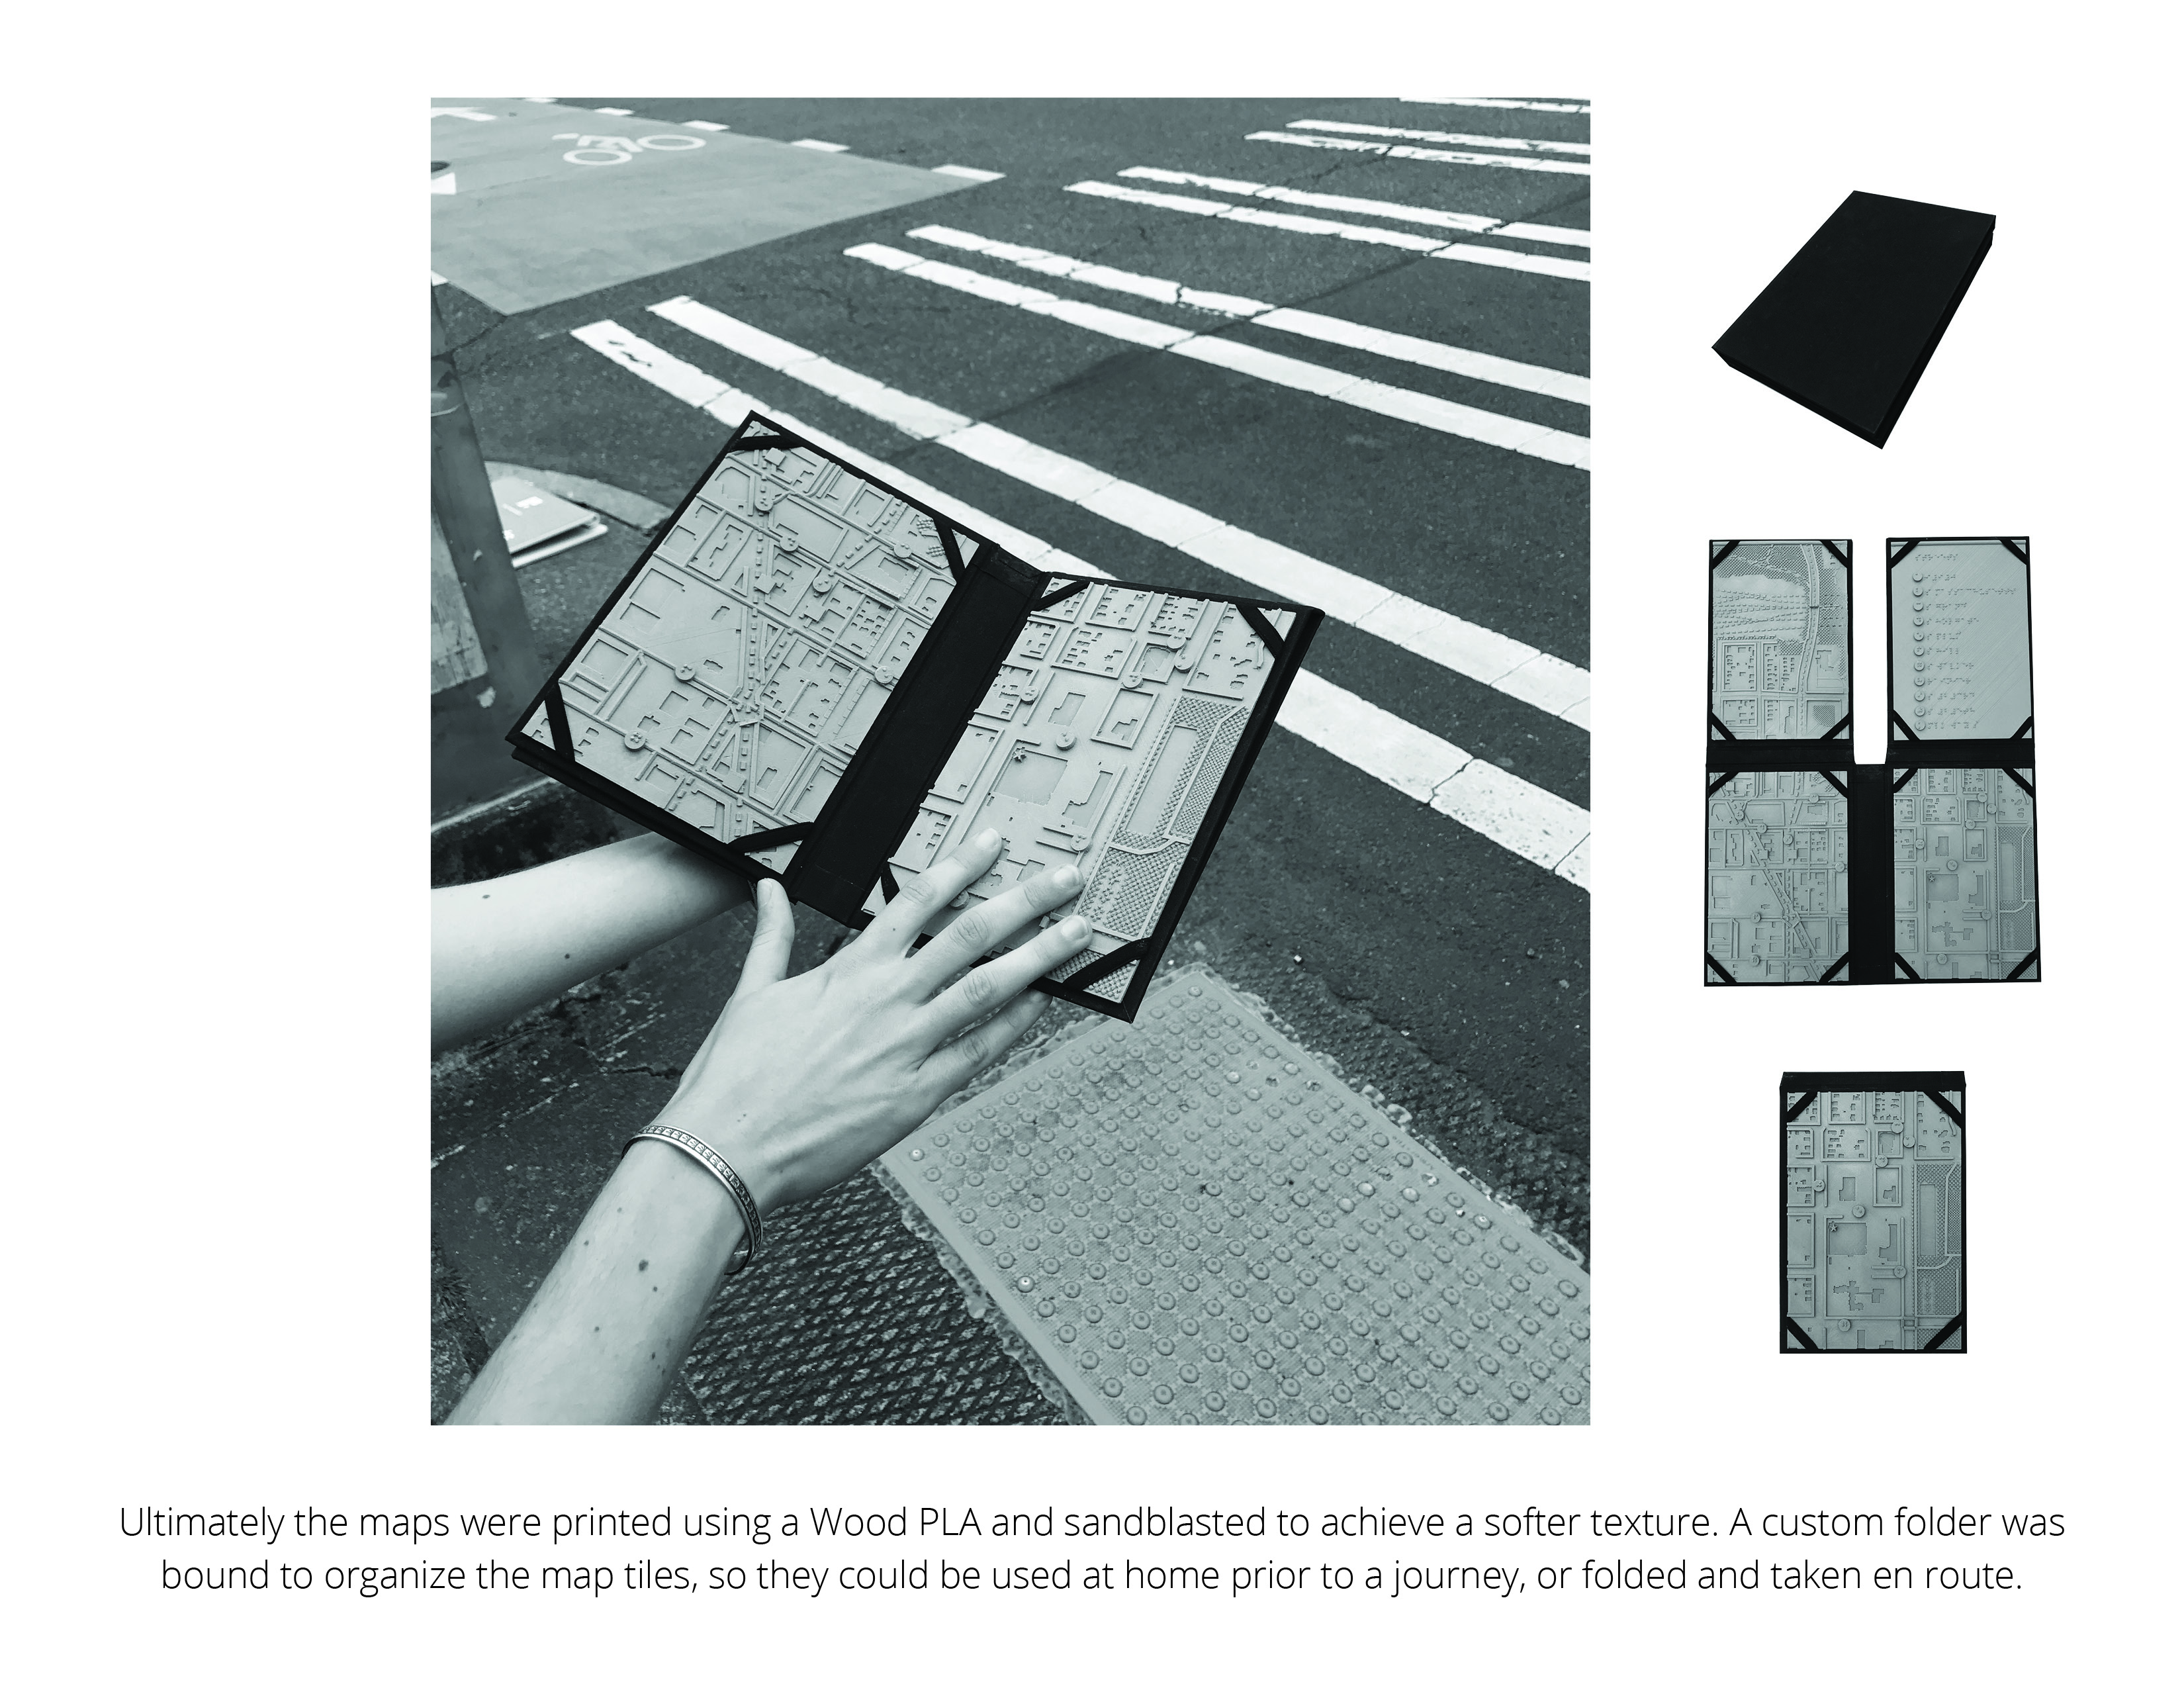
\includegraphics[width=5in]{pics/ProjPilot.jpg}
    \caption{Tactile Maps Generated Via Preliminary Study}
    \label{fig:pilot}
\end{figure}


The map tiles were produced for two areas in Seattle that would be familiar to our users.
Due to 3D print bed constraints, map tiles were limited to ~8” x 5.5”.  The map was scaled such that 1”=200’ (1mm=2.4m). This scale accommodated an area roughly 3x4 blocks. In order to capture an area that includes both the forthcoming Judkins Park Transit Station, and Seattle Lighthouse for the Blind at this scale 3 tiles were needed.   

Based on preliminary feedback from expert users, basic features of the urban pedestrian environment were legible at this scale.  Further usability testing and symbol development must be conducted in order to confidently say if this scale is appropriate as a navigational aid.   The case study map series was printed with slight variation in symbol style, and size on each tile in anticipation of user testing, however it seems likely that the variations produced were not adequately different and should be exaggerated more for future testing.

Appendix C map features printed with measurements.
Experts interviewed indicated a more detailed tactile representation of smaller sites might also be valuable.  Potential areas cited that would benefit from the availability of detailed maps include transit stations, and complex intersections, particularly non-perpendicular intersections and those involving the junction of three or more streets.  Additional interviews or a survey distributed more broadly would be useful in identifying other areas of interest, and what features of these spaces should be prioritized for representation.  

There is an additional opportunity to apply the approach used in this project to developing maps that convey different types of information.  Zoomed way out, it would be relatively easy to create maps that are more reflective of the broader context of an area or district.  Here again there is an opportunity to create a basic symbol set for features that would be desirable in order to better understand how an area is situated in place.  In addition to the standard cartographic information such as scale and cardinal direction, this may include green spaces, water bodies, arterials, district lines, etc.  


We conducted a  preliminary study in a focus group meeting of 27 Deaf-blind individuals to assess need. We asked participants to explain how they travel and the issues most troublesome to them. 
Our study aimed to better understand how Deaf-blind people currently access community travel and 
accommodate inaccessibility in the built environment. In addition we were interested to know whether a tangible map we 3D printed for the area in which the participants met us added to their overall knowledge and confidence about traveling in that neighborhood.


%We first asked the participants to meet us at the public library where the Deaf-blind Service Center organizes community events. 
%We observed their arrival to the library location. 
Of the participants in the focus group, four individuals agreed to participate in semi-structured interviews at a public library location familiar to them. We asked about their travel habits and strategies for using inaccessible built environments.
Participants conversed with us through  interpreted sign language, and the whole session was video recorded. %, they would interrupt the exploration session to explain to us what they understood about the map.

\textbf{“I don’t see anything and I feel limited in independence. I walk the same route that I’m used to that I’ve learned. If I moved to a new place I wouldn’t be able to go out. ... I feel limited where I can go and I can’t go outside by myself."}

Our interviews highlighted the need to support increased independence. All but one participant indicated they asked for help from a friend or a stranger in their travel to the meeting location. %: frequently seeking help created a perceived social burden. Furthermore, p
However, participants were concerned about creating a burden for helpers and worried that someone may not be available when they most needed it. 
%Many indicated it is important for them to find alternate solutions that can increase the independence of the Deaf-blind in their daily lives.
Participants also mentioned the difficulty of learning about changes in the environment such as new building. One said: %\item Participants felt that their city was becoming harder to access because the terrain is changing so fast. At first, they were surprised to learn via our tactile map about the new buildings and other changes to the environment. Some expressly voiced frustrations, 
``...landmarks are disappearing! I thought this was there and now it is not. Now it is a big multi level building!''

We presented the participants a tactile map of the area in which we met them and asked participants to survey the tactile map. We asked them to find the location of the library in which we met, which was signified by a \textit{landmark} tactile icon, as shown in Figure \ref{fig:pilot}. We asked participants to explore the area and note any items, landmarks, street-names, buildings, bus stops or features that they understood to be in the area their hands were exploring. %We observed the manner in which they explored the map and recorded their exploration via video. %It should be noted that since individuals were conversing 

%We extracted the following key insights, which we will use to inform the design of this development project and we will also factor directly into the production of parsimonious yet useful tactile representations on the maps:



With regard to the design of the tactile map, participants highlighted the importance of choosing good ways to convey information. For example, Braille was ``sharp to the touch'' and difficult to interpret without memorizing abbreviations due to limited space. Providing tactile maps with the right details, at the right density and frequency is crucial. For example, participants found it confusing when there was no tactile information when their finger was inside a large park. In other places, participants found the features to be too dense to distinguish. This brings up one of our main design challenges, e.g., the granularity and density of tactile presentation.

Participants also asked about how one can obtain these tactile maps, where one would go to print them, and how much they cost. They were interested in understanding the interface with which they would create these maps, and how they would print them. This highlights the importance of building not just the tactile maps right, but also the interfaces that the users will interact with should be accessible to the Deaf-blind users.

%\\item Labeling maps with Braille seemed a straightforward solution to us, but participants non-uniformly understood the abbreviations we used and some indicated discomfort with the 3D printed Braille that was produced via additive manufacturing, indicating it was too sharp to the touch.
%\item Participants found it difficult to do anything else when holding the map in one hand, tucking their cane under one arm and reading the tactile map with the other hand. In an actual travel scenario, such
%difficulty might result in loss of orientation, thus interrupting
%the travel task and potentially causing confusion and frustration.
%\end{itemize}


\ac{
reconcile SK list above with JM list below
\begin{itemize}
\item We will develop a map creation tool that uses multi-variable optimization algorithms to balance information richness with tactile usability (appropriate use and density of tactile real estate). Our optimization cost functions will be designed to accommodate the user’s requirements about the area of travel, type of travel, and user needs and preferences (taking a parameterized approach).  To support this, we will will use the OpenSidewalks pedestrian-centric data standard and \ac{citation} standard tactile symbols to represent features in a replicable, pedestrian-appropriate manner. (Described in Section~\ref{sec:optimize}).
\item  We will build an accessible, user-friendly product that is integrated into our  production-level accessible map, designing all exchanges to be easily navigable  using a 14 cell portable Braille reader (the most constrained interface we know to be in use)  (Described in Section~\ref{sec:accessmap-extension}).
\item We will validate our map creation tool and end-to-end interaction product in an iterative, user-centered fashion, as described in Section~\ref{sec:mapping-validation} and Section~\ref{sec:accessmap-studies}, respectively. 
\end{itemize}
}
